\section{Database}
Si è scelto di utilizzare un database relazionale per 
la gestione dei dati dell'applicazione.
Come database è stato scelto PostgreSQL.

\subsection{Schema del Database}
\subsubsection{Diagramma Entità-Relazione}
Il database è stato progettato realizzando un 
diagramma Entità-Relazione che racchiude i dati che si ritiene 
necessario gestire.
\begin{figure}[H]
  \centering
  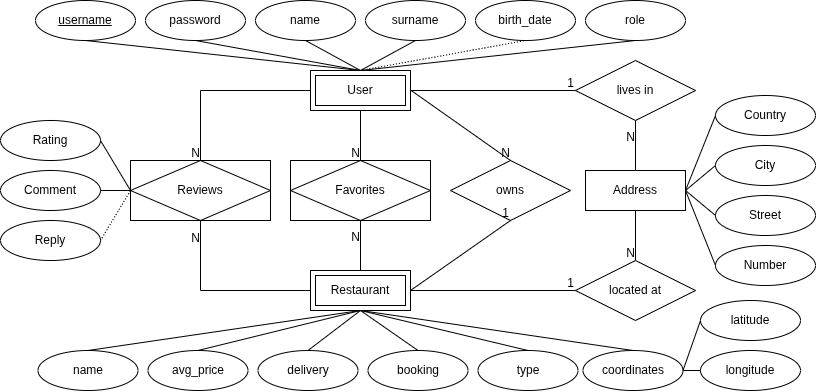
\includegraphics[width=\textwidth]{images/ER-base.png}
  \caption{Diagramma ER}
  \label{fig:er-diagram}
\end{figure}
Come si evince dal diagramma l'entità principale 
è \textit{Address} che contiene i dati relativi agli indirizzi. 
\textit{User} e \textit{Restaurant} sono in relazione con \textit{Address} 
e a loro volta sono in relazione tra loro.
\textit{Review} e \textit{Favorite} sono entità che collegano 
\textit{User} e \textit{Restaurant} per gestire le recensioni
e i ristoranti preferiti dagli utenti.
\subsubsection{Rielaborazione del Diagramma}
Successivamente è stata eseguita una rielaborazione del diagramma
per normalizzare le tabelle.
\begin{figure}[H]
  \centering
  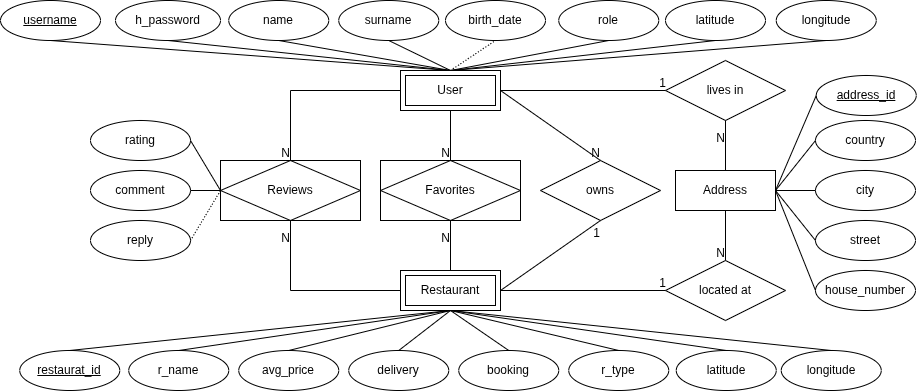
\includegraphics[width=\textwidth]{images/ER-refactored.png}
  \caption{Diagramma ER Normalizzato}
  \label{fig:er-diagram2}
\end{figure}
Dopo questa rielaborazione le coordinate da attributo derivato 
sono diventati attributi semplici.
Tuttavia, nell'implementazione finale, si è deciso di spostare le 
coordinate nell'entità \textit{Address} per una migliore gestione.
\subsubsection{Schema}
Infine si sono elencate le tabelle e i relativi attributi:
\begin{itemize}
    \item \textbf{addresses} (\underline{address\_id}, country, city, street, house\_number, latitude, longitude)
    \item \textbf{users} (\underline{username}, h\_password, name, surname, birth\_date, role, address\_id\textsuperscript{addresses})
    \item \textbf{restaurants} (\underline{restaurant\_id}, r\_owner, r\_name, avg\_price, delivery, booking, r\_type, address\_id\textsuperscript{addresses})
    \item \textbf{favorites} (\underline{username\textsuperscript{users}, restaurant\_id\textsuperscript{restaurants}})
    \item \textbf{reviews} (\underline{username\textsuperscript{users}, restaurant\_id\textsuperscript{restaurants}}, rating, comment, reply)
\end{itemize}
Questa lista delle tabelle è stata infine implementata nel database.

\subsection{Tabelle}
\subsubsection{Addresses}
La tabella \textit{addresses} contiene gli indirizzi degli 
utenti e dei ristoranti.\\
Gli attributi sono:
\begin{itemize}
    \item \textbf{address\_id}: identificativo univoco dell'indirizzo
    \item \textbf{country}: nazione
    \item \textbf{city}: città
    \item \textbf{street}: via
    \item \textbf{house\_number}: numero civico
    \item \textbf{latitude}: latitudine
    \item \textbf{longitude}: longitudine
\end{itemize}
Sono stati posti dei vincoli di integrità per garantire che 
le coordinate siano valide, nello specifico che la latitudine
sia compresa tra -90 e 90 e la longitudine tra -180 e 180.

\subsubsection{Users}
La tabella \textit{users} contiene gli utenti registrati 
nell'applicazione.\\
Gli attributi sono:
\begin{itemize}
    \item \textbf{username}: identificativo univoco dell'utente
    \item \textbf{h\_password}: password in hash
    \item \textbf{name}: nome
    \item \textbf{surname}: cognome
    \item \textbf{birth\_date}: data di nascita
    \item \textbf{role}: ruolo dell'utente (owner o client)
    \item \textbf{address\_id}: identificativo dell'indirizzo dell'utente
\end{itemize}
Il campo \textit{role} è stato implementato creando un tipo di 
dato enumerativo che può assumere i valori \textit{owner} o \textit{client}.\\
Il campo \textit{h\_password} prevede che la password venga 
memorizzata in forma di hash per garantire la sicurezza.
Si è scelto di utilizzare l'algoritmo di hashing 
\href{https://github.com/p-h-c/phc-winner-argon2}{Argon2} suggerito 
da \href{https://cheatsheetseries.owasp.org/cheatsheets/Password_Storage_Cheat_Sheet.html}{OWASP}.\\
Il campo \textit{address\_id} è una chiave esterna che fa riferimento 
alla tabella \textit{addresses}. 
In caso di modifica dell'indirizzo
di un utente, si aggiornerà il campo \textit{address\_id}, in caso 
di cancellazione dell'indirizzo non verrà cancellato l'utente.

\subsubsection{Restaurants}
La tabella \textit{restaurants} contiene i ristoranti creati 
dai ristoratori.\\
Gli attributi sono:
\begin{itemize}
    \item \textbf{restaurant\_id}: identificativo univoco del ristorante
    \item \textbf{r\_owner}: proprietario del ristorante (username dell'utente)
    \item \textbf{r\_name}: nome del ristorante
    \item \textbf{avg\_price}: prezzo medio del ristorante inserito dal ristoratore
    \item \textbf{delivery}: servizio di consegna disponibile (booleano)
    \item \textbf{booking}: servizio di prenotazione disponibile (booleano)
    \item \textbf{r\_type}: tipo di cucina del ristorante (es. cinese, italiano, etc.)
    \item \textbf{address\_id}: identificativo dell'indirizzo del ristorante
\end{itemize}
Il campo \textit{r\_owner} è una chiave esterna che fa riferimento
alla tabella \textit{users} e rappresenta il proprietario del ristorante.
In caso di moifica di \textit{username} dell'utente, si aggiornerà
il campo \textit{r\_owner}, in caso di cancellazione dell'utente 
verrà cancellato anche il ristorante.\\
Il campo \textit{address\_id} è una chiave esterna che fa riferimento
alla tabella \textit{addresses}.
In caso di modifica dell'indirizzo del ristorante, si aggiornerà
il campo \textit{address\_id}, in caso di cancellazione dell'indirizzo
non verrà cancellato il ristorante.\\
\`E stato posto un vincolo di integrità per garantire che il
prezzo medio sia un numero positivo.

\subsubsection{Favorites}
La tabella \textit{favorites} server a gestire i 
ristorante preferiti dagli utenti.\\
Gli attributi sono:
\begin{itemize}
    \item \textbf{username}: identificativo dell'utente
    \item \textbf{restaurant\_id}: identificativo del ristorante
\end{itemize}
Il campo \textit{username} è una chiave esterna che fa riferimento
alla tabella \textit{users} e il campo \textit{restaurant\_id} 
è una chiave esterna che fa riferimento
alla tabella \textit{restaurants}. In caso di modifica dei due campi
si aggiorneranno i rispettivi campi, in caso di cancellazione
di un utente o di un ristorante, verrà cancellata la preferenza.

\subsubsection{Reviews}
La tabella \textit{reviews} serve a gestire le recensioni
che gli utenti possono lasciare ai ristoranti.\\
Gli attributi sono:
\begin{itemize}
    \item \textbf{username}: identificativo dell'utente
    \item \textbf{restaurant\_id}: identificativo del ristorante
    \item \textbf{rating}: valutazione da 1 a 5
    \item \textbf{comment}: commento della recensione
    \item \textbf{reply}: risposta del ristoratore alla recensione
\end{itemize}
Il campo \textit{username} è una chiave esterna che fa riferimento
alla tabella \textit{users} e il campo \textit{restaurant\_id} 
è una chiave esterna che fa riferimento
alla tabella \textit{restaurants}. In caso di modifica dei due campi
si aggiorneranno i rispettivi campi, in caso di cancellazione
di un utente o di un ristorante, verrà cancellata la recensione.\\
Sul \textit{rating} è stato posto un vincolo di integrità
per garantire che sia un numero intero compreso tra 1 e 5.
